\chapter{COFFEE: a Compiler for Fast Expression Evaluation}
\label{ch:coffee}

\section{Overview}
Sharing elimination and pre-evaluation, which we presented in Chapter~\ref{ch:optimality}, as well as the low level optimizations discussed in Chapter~\ref{ch:lowlevelopt}, have been implemented in COFFEE\footnote{COFFEE is the acronym for COmpiler For Fast Expression Evaluation.}, a mature, platform-agnostic compiler. COFFEE has fully been integrated with Firedrake, the framework based on the finite element method introduced in Section~\ref{sec:bkg:firedrake}. The code, which comprises more than 5000 lines of Python, is available at~\citep{coffee-code}.

Firedrake users employ the Unified Form Language to express problems in a notation resembling mathematical equations. At run-time, the high-level specification is translated by a form compiler, the Two-Stage Form Compiler (TSFC)~\cite{TSFC-Compiler}, into one or more abstract syntax trees (ASTs) representing assembly kernels. ASTs are then passed to COFFEE for optimization. The output of COFFEE, C code, is eventually provided to PyOP2~\citep{pyop2isc}, where just-in-time compilation and execution over the discretized domain take place. The flow and the compiler structure are outlined in Figure~\ref{fig:coffee-pipeline}. 

\begin{figure}
\centering
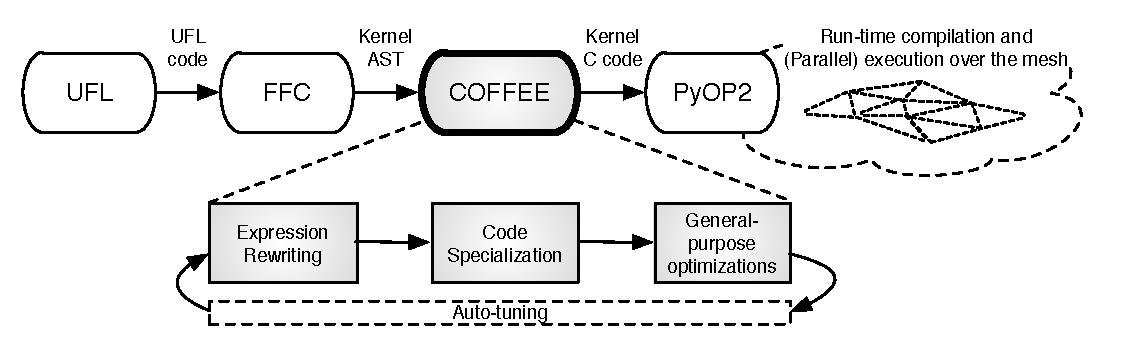
\includegraphics[scale=0.50]{coffee/pictures/coffee-pipeline.pdf}
\caption{The structure of COFFEE and its place within Firedrake.}
\label{fig:coffee-pipeline}
\end{figure}

\section{The Compilation Pipeline}
\label{sec:coffee:pipeline}
Similarly to general-purpose compilers, COFFEE provides different optimization levels, namely \texttt{O0}, \texttt{O1}, \texttt{O2} and \texttt{O3}. Apart from \texttt{O0}, which does not transform the code received from the form compiler (useful for debugging purposes), all optimization levels apply ordered sequences of optimizations. In essence, the higher the optimization level, the more aggressive (and potentially slower) is the transformation process. In the following, when describing aspects of the optimization process common to \texttt{O1}, \texttt{O2} and \texttt{O3}, we will use the generic notation \texttt{Ox} (\texttt{x} $\in \lbrace 1, 2, 3\rbrace$).

The optimization level \texttt{Ox} can logically be split into three phases:
\begin{description}
\item[Expression rewriting] Any transformation changing the structure of the expressions in the assembly kernel belongs to this class. For example, a high level optimization (sharing elimination, pre-evaluation) or, more in general, any rewrite operator (described later in Section~\ref{sec:coffee:rewrite-ops}) such as generalized code motion or factorization. 
\item[Handling of block-sparse tables] Explained in Section~\ref{ch:optimality:block-sparse}, this phase consists of restructuring the iteration spaces searching for a trade-off between the avoidance of useless operations involving blocks of zeros in basis function tables and the effectiveness of low level optimization.
\item[Code Specialization] The class of low level optimizations. The primary focus of this thesis has been code specialization for conventional CPUs, although a generalization to other platforms is possible. In this phase, a specific combination of the transformations presented in Chapter~\ref{ch:coffee} is applied.
\end{description}
These three phases are totally ordered. Expression rewriting introduces temporaries and creates loops. All loops, including those produced by expression rewriting, and the statements therein are potentially transformed in the subsequent phase, by adjusting bounds and introducing memory offsets, respectively. The output of the first two phases is finally processed for padding and data alignment, vector-register tiling and vector promotion.

\paragraph{Phase 1: analysis}
During the analysis phase, an AST is visited and several kinds of information are collected. In particular, COFFEE searches for expression rewriting candidates. These are represented by special nodes in the AST, which we refer to as ``expression nodes''. In plain C, we could think of an expression node as a statement preceded by a directive such as \texttt{$\#$pragma coffee expression}; the purpose of the directive would be to trigger COFFEE's \texttt{Ox}. This is for example similar to the way loops are parallelized through OpenMP. If at least one expression node is found, we proceed to the next phase, otherwise the AST is unparsed and C code returned.

\paragraph{Phase 2: checking legality}
In addition to \texttt{Ox}, users can craft their own custom optimization pipelines by composing the individual transformations available in COFFEE. However, since some of the low level transformations are inherently not composable (e.g., loop unrolling with vector-register tiling), the compiler always checks the legality of the transformation sequence. 

\paragraph{Phase 3: AST transformation}
If the sequence of optimizations is legal, the AST is processed. In particular:
\begin{description}
\item[\texttt{O1}] At lowest optimization level, expression rewriting reduces to generalized code motion, while only padding and data alignment are applied among the low level optimizations.
\item[\texttt{O2}] With respect to \texttt{O1}, there is only one yet fundamental change: expression rewriting now performs sharing elimination (i.e., Algorithm~\ref{algo:sharing-elimination}).
\item[\texttt{O3}] Algorithm~\ref{algo:gamma}, which coordinates sharing elimination and pre-evaluation, is applied. This is followed by handling block-sparse tables, and finally by padding and data alignment. 
\end{description}

\paragraph{Phase 4: code generation}
Once all optimizations have been applied, the AST is visited one last time and a C representation (a string) is returned.

\section{Plugging COFFEE into Firedrake}
\label{sec:coffee-implementation}

\subsection{Abstract Syntax Trees}
In this section, we highlight peculiarities of the hierarchy of AST nodes.

\paragraph{Special nodes}
Firstly, we observe that some nodes have special semantics. The expression nodes described in the previous section is one such example. A whole sub-hierarchy of \texttt{LinAlg} nodes is available, with objects such as \texttt{Invert} and \texttt{Determinant} representing basic linear algebra operation. Code generation for these objects can be specialized based upon the underlying architecture and the size of the involved tensors. For instance, a manually-optimized loop nest may be preferred to a BLAS function when the tensors are small\footnote{It is well-known that BLAS libraries are highly optimized for big tensors, while their performance tends to be sub-optimal with small tensors, which are very common in assembly kernels.}. Another special type of node is \texttt{ArrayInit}, used for static initialization of arrays. An \texttt{ArrayInit} wraps an N-dimensional Numpy array~\citep{Numpy} and provides a simple interface to obtain information useful for optimization, like the sparsity pattern of the array. 

\paragraph{Symbols}
A \texttt{Symbol} represents a variable in the code. The \textit{rank} of a \texttt{Symbol} captures the dimensionality of a variable, with a rank equal to $N$ indicating that a variable is an $N$-D array ($N=0$ implies that the variable is a scalar). The rank is implemented as an $N$-tuple, each entry being either an integer or a string representing a loop dimension. The \textit{offset} of a \texttt{Symbol} is again an $N$-tuple where each element is a 2-tuple. For each entry $r$ in the rank, there is a corresponding entry ${<}scale,\ stride{>}$ in the offset. Rank and offset are used as in Figure~\ref{fig:coffee-ast-vs-c} to access specific memory locations. By clearly identifying rank and offset of a \texttt{Symbol} -- rather than storing a generic expression -- the complexity of the data dependency analysis required by the rewrite operators is greatly reduced. The underlying assumption, however, is that all symbols in the kernel (at least those relevant for optimization) have access functions (see Section~\ref{sec:bkg:terminology}) that are affine in the loop indices. As motivated in Chapter~\ref{ch:optimality}, this is definitely the case for the class of kernels in which we are interested.

\begin{figure}
\begin{center}
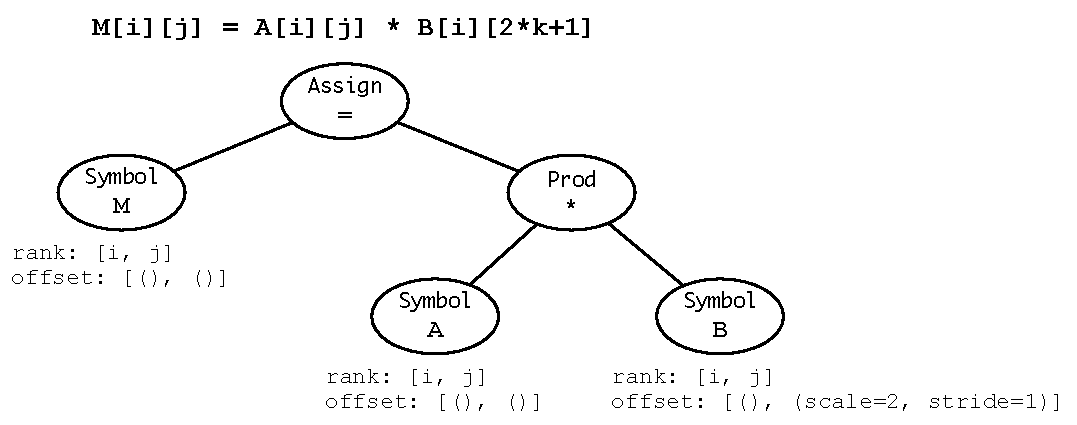
\includegraphics[scale=0.70]{coffee/pictures/coffee-ast.pdf}
\caption{AST representation of a C assignment in COFFEE.}
\label{fig:coffee-ast-vs-c}
\end{center}
\end{figure}

\paragraph{Building an AST}
Rather than using a parser, COFFEE exposes to the user the whole hierarchy of nodes for explicitly building ASTs. This is because the compiler is meant to be used as an intermediate step in a multilayer framework based on DSLs. To ease the construction of ASTs (especially nested loops), a set of utility functions is provided. We will elaborate on these aspects in the next section.

\subsection{Integration with Form Compilers}
So far, COFFEE has been integrated with two form compilers: the FEniCS Form Compiler (FFC) and the Two-Stage Form Compiler (TSFC)\footnote{The generation of ASTs in TSFC has been written by Myklos Homolya.}. These form compilers have their own internal representation of an assembly kernel; the objective is to turn such a representation into an AST suitable for COFFEE. We here describe how we achieved this in the case of FFC.

The key idea is to enrich the FFC's intermediate representation at construction time; that is, when the UFL specification of a form is translated. We made the following changes.
\begin{itemize}
\item The mathematical expression evaluating the element tensor is represented as a tree data structure, or ``FFC-AST''. A limitation of an FFC-AST was that its nodes -- symbols or arithmetic operations -- were not bound to loops. For instance, the FFC-AST node corresponding to the symbol \texttt{A[i][j]} did not separate the variable name \texttt{A} from the loop indices \texttt{i} and \texttt{j}. We have therefore enriched FFC-AST symbols with additional fields to capture these information.
\item Basis functions in an FFC-AST are added a new field storing the dimensionality of their function space. This information is used to enrich \texttt{ArrayInit} objects with the sparsity pattern of the values they are representing (recall that the tabulation of vector-valued basis functions is characterized by the presence of zero-valued blocks).
\end{itemize}

The improved FFC-AST is intercepted prior to code generation (the last phase in the original FFC, which outputs C code directly) and forwarded to a new module, where a COFFEE AST is finally built. In this module:
\begin{itemize}
\item the template originally used by FFC for code generation (i.e., the parts of an assembly kernels that are immutable across different forms) is changed in favour of ``static'' pieces of AST (kernel signature, loop nests, etc).
\item the FFC-AST is visited and translated into a COFFEE AST by a suitable AST-to-AST converter routine.
\end{itemize}

The Two-Stage Form Compiler was originally conceived to produce ASTs for COFFEE, so no particular changes to its intermediate representation were needed. 


\section{Rewrite Operators}
\label{sec:coffee:rewrite-ops}
COFFEE implements sharing elimination and pre-evaluation by composing ``building-block'' operators, or ``rewrite operators''. This has several advantages. Firstly, extendibility: novel transformations -- for instance, sum-factorization in spectral methods -- could be expressed using the existing operators, or with small effort building on what is already available. Secondly, generality: COFFEE can be seen as a lightweight, low level computer algebra system, not necessarily tied to finite element integration. Thirdly, robustness: the same operators are exploited, and therefore stressed, by different optimization pipelines. The rewrite operators, whose implementation is based on manipulation of the kernel's AST, essentially compose the COFFEE language. 

The most important rewrite operators in COFFEE are:
\begin{description}
\item[Generalized code motion] It pre-computes the values taken by a sub-expression along an invariant dimension. This is implemented by introducing a temporary array per invariant sub-expression and by adding a new ``clone'' loop to the nest (Several examples, e.g. Figure~\ref{code:loopnest}, have been provided throughout the thesis). At the price of some extra memory for storing temporaries, all lifted terms are now amenable to auto-vectorization. 
\item[Expansion] This transformation consists of expanding (i.e., distributing) a product between two generic sub-expressions. Expansion has several effects, the most important ones being exposing factorization opportunities and increasing the operation count. It can also help relieving the register pressure within a loop, by allowing further code motion.
\item[Factorization] Collecting, or factorizing, symbols reduces the number of multiplications and potentially exposes, as illustrated through sharing elimination, code motion opportunities.
\item[Symbolic evaluation] This operator evaluates sub-expressions that only involve statically initialized, read-only arrays (e.g., basis function tables). The result is stored into a new array, and the AST modified accordingly
\end{description}
All these operators are used by both sharing elimination and pre-evaluation (apart from symbolic evaluation, only employed by pre-evaluation).

The rewrite operators accept a number of options to drive the transformation process. With code motion, for example, we can specify what kind of sub-expressions should be hoisted (by indicating the expected invariant loops) or the amount of memory that is spendable in temporaries. Factorization can be either ``explicit'', by providing a list of symbols to be factorized or a loop dimension along which searching for factorizable symbols, or ``heuristic'', with the algorithm searching for the groups of most recurrent symbols.

\section{Features of the Implementation}
Rather than providing the pseudo-code and an explanation for each of the algorithms implemented in COFFEE -- a mere exercise of scarce interest for the reader, given that the implementation is open-source and well-documented -- this section focuses on the structure of the compiler and its ``toolkit'' for implementing or extending rewrite operators.

\subsection{Tree Visitor Pattern}
The need for a generic infrastructure for traversing ASTs has grown rapidly, together with the complexity of the compiler. In the early stages of COFFEE, any time that a new transformation (e.g., a rewrite operator) or data collector (e.g., for dependence analysis) were required, the full AST traversal had to be (re-)implemented. In addition, the lack of a common interface for tree traversals made the code more difficult to understand and to extend. This led to the introduction of a tree visitor design pattern\footnote{The tree visitor infrastructure was mainly developed by Lawrence Mitchell, and was inspired by that adopted in UFL, the language used to specify forms in Firedrake.}, whose aim is to decouple the algorithms from the data structure on which they are applied~\cite{wiki-tree-visitors}. 

Consider, without loss of generality, an algorithm that needs to perform special actions (e.g., collecting loop dependence information) any time a \texttt{Symbol} or a \texttt{ForLoop} nodes are encountered. Then, a tree visitor will only need to implement three methods, namely \texttt{visit$\_$Symbol} and \texttt{visit$\_$ForLoop} -- the actual handlers -- as well as \texttt{visit$\_$Node}, which implements the ``fallback'' action for all other node types (typically, just a propagation of the visit).

Tree visitors exploit the hierarchy of AST nodes by always dispatching to the most specialized handler. For example, symbols are simultaneously of type \texttt{Symbol} and \texttt{Expression}, but if a \texttt{Symbol} is encountered and \texttt{visit$\_$Symbol} is implemented, then \texttt{visit$\_$Symbol} is executed, whereas \texttt{visit$\_$Expression} (if any) is ignored.

Most of the algorithms in COFFEE exploit the tree visitor pattern; a few, the ``oldest'' ones, still do not, due to the lack of time for porting to the new infrastructure.

\subsection{Flexible Code Motion}
\label{sec:coffee:cm}
Code motion consists of lifting, or hoisting, a (sub-)expression out of one or more loops. This rewrite operator is used in many different contexts: as a stand-alone transformation (optimization level \texttt{O1}); in multiple steps during sharing elimination; in pre-evaluation. 

When applying the operator, several pieces of information must be known:
\begin{enumerate}
\item What sub-expression should be hoisted; for instance, should they be constant in the whole loop nest or invariant in at most one of the linear loops.
\item Where to hoist it; that is, how many loops is the operator allowed to cross.
\item How much memory are we allowed to use for a temporary.
\item If a common sub-expression had already been hoisted.
\end{enumerate}
The code motion operator is flexible and let the caller (i.e., a higher-level transformation) drive the hoisting process by specifying how to behave with respect to the aforementioned points.

COFFEE must therefore track all of the hoisted sub-expressions for later retrieval. A dictionary mapping each of the temporaries introduced to a tuple of metadata is employed. For a temporary \texttt{t}, the dictionary records:
\begin{itemize}
\item A reference to the hoisted expression \texttt{e} assigned to \texttt{t}.
\item A reference to the loop in which \texttt{e} is lifted.
\item A reference to the declaration of \texttt{t}.
\end{itemize}
This dictionary belongs to the ``global state'' of COFFEE. It is updated each time the code motion operator is invoked, and read by other transformations (e.g., by all of the lower level optimizations).

The code motion operator ``silently'' applies common sub-expression elimination. A look-up in the dictionary tells whether a hoistable sub-expression \texttt{e} has been assigned to a temporary \texttt{t} by a prior call to the operator; in such a case, \texttt{e} is straightforwardly replaced with \texttt{t}, that is, no further temporaries are introduced. 

%The code motion operator is ``smart'', in the sense that common sub-expressions,  every time a sub-expression is about to be hoisted, \texttt{e} is lifted out of the iteration space \texttt{I}, three further ``extra'' optimizations are attempted. 
%
%\begin{description}
%\item[Identification of common sub-expression] If a semantically equivalent sub-expression \texttt{e'} had been hoisted along the same iteration space \texttt{I}, then \texttt{e} is rather replaced with a reference to the temporary that \texttt{e'} is assigned to.
%\item[Loop fusion.] When test and trial functions belong to the same function space, common sub-expressions may arise over different loops.  


\subsection{Tracking Data Dependency}
Data dependency analysis is necessary to ensure the legality of some transformations. For example:
\begin{itemize}
\item When lifting a sub-expression \texttt{e}, we may want to hoist ``as far as possible'' in the loop nest (possibly even outside of it); that is, right after the last write to a variable read in \texttt{e}.
\item When expanding a product, some terms may be aggregated with previously hoisted sub-expressions. This would avoid introducing extra temporaries and increasing the register pressure. For example, if we have \texttt{(a + b)*c} and both \texttt{a} and \texttt{b} are temporaries created by code motion, we could expand the product and aggregate \texttt{c} with the sub-expressions stored by \texttt{a} and \texttt{b}. Obviously, this is as long as neither \texttt{a} nor \texttt{b} are accessed in other sub-expressions.
\item For loop fusion (see Section~\ref{sec:coffee-loopfusion}).
\end{itemize}

In a similar way to general-purpose compilers, COFFEE uses a dependency graph for tracking data dependencies. The dependency graph has as many vertices as symbols in the code; a direct edge from \texttt{A} to \texttt{B} indicates that symbol \texttt{B} depends on (i.e., is going to read) symbol \texttt{A}. Since COFFEE relies on \textit{static single assignment} -- a property that ensures that variables are assigned exactly once -- such a minimalistic data structure suffices for data dependence analysis.

\subsection{Minimizing Temporaries}
Both code motion operator (Section~\ref{sec:coffee:cm}) and common sub-expression elimination induced by loop fusion (Section~\ref{sec:coffee-loopfusion}) impact the number of temporaries in the assembly kernel. At the end of expression rewriting, a routine in COFFEE attempts to remove all of the unnecessary temporaries. This makes the code more readable and, potentially, relieves the register pressure.

The main rule for removing a temporary \texttt{t} storing an expression \texttt{e} is that if \texttt{t} is accessed only in a single statement \texttt{s}, then \texttt{e} is inlined into \texttt{s} and \texttt{t} is removed. Secondly, if some of the transformations in the optimization pipeline reduced \texttt{e} to a symbol, then any appearance of \texttt{t} is also replaced by \texttt{e}.